\documentclass{standalone}
\usepackage{tikz}
\usepackage{animate}
\usepackage{amsmath}
\usepackage{ifthen}
\usetikzlibrary {matrix}
\usepackage{tikzlings}
\usepackage{tikzlings-penguins}

\begin{document}
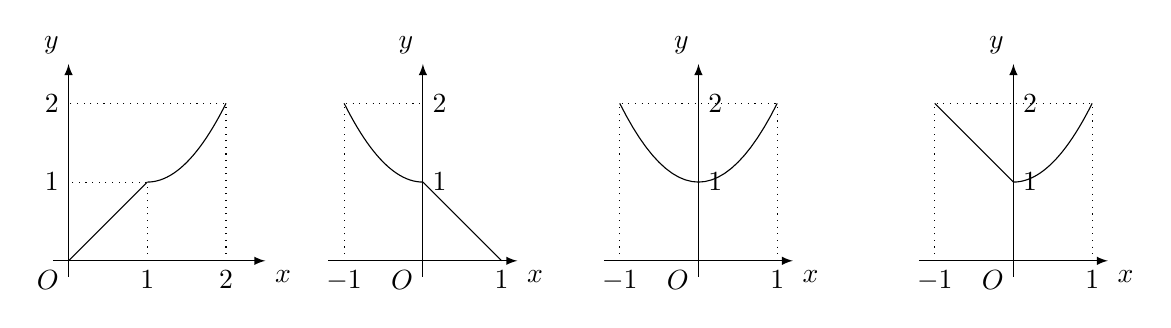
\begin{tikzpicture}[>=latex]
  \begin{scope}
    \draw[->] (-0.2,0) --(2.5,0) node[below right] {$x$};
    \draw[->] (0,-0.2) --(0,2.5) node[above left]  {$y$};
    \draw[domain=0:1] plot (\x,\x);
    \draw[domain=1:2] plot (\x,{(\x-1)*(\x-1)+1});
    \draw[dotted] (1,0)--(1,1)--(0,1);
    \draw[dotted] (2,0)--(2,2)--(0,2);
    \node[below left]  (o) at (0,0) {$O$};
    \foreach \x in {1,2}{
      \node[below] (x\x) at (\x,0) {$\x$};
      \node[left] (y\x) at (0,\x) {$\x$};
    }
  \end{scope}
  \begin{scope}[xshift=4.5cm]
    \draw[->] (-1.2,0)--(1.2,0) node[below right] {$x$};
    \draw[->] (0,-0.2)--(0,2.5) node[above left] {$y$};
    \draw[domain=0:1] plot (\x,1-\x); 
    \draw[domain=-1:0] plot(\x,{\x*\x+1});
    \draw[dotted] (-1,0)--(-1,2)--(0,2);
    \node[below left]  (o) at (0,0) {$O$};
    \foreach \x in {-1,1} 
    {
     \node[below] at (\x,0) {$\x$}; 
    }
    \foreach \x in {1,2} 
    \node [right] at (0,\x) {$\x$};
  \end{scope}
  \begin{scope}[xshift=8cm]
    \draw[->] (-1.2,0)--(1.2,0) node [below right] {$x$};
    \draw[->] (0,-0.2) --(0,2.5) node[above left] {$y$};
    \draw[domain=-1:1] plot (\x,{\x*\x+1});
    \draw[dotted] (-1,0)--(-1,2)--(1,2)--(1,0);
    \node[below left]  (o) at (0,0) {$O$};
    \foreach \x in {-1,1} 
    {
     \node[below] at (\x,0) {$\x$}; 
    }
    \foreach \x in {1,2} 
    \node [right] at (0,\x) {$\x$};
  \end{scope}
  \begin{scope}[xshift=12cm]
    \draw[->] (-1.2,0)--(1.2,0) node [below right] {$x$};
    \draw[->] (0,-0.2) --(0,2.5) node[above left] {$y$};
    \draw[domain=0:1] plot (\x,{\x*\x+1});
    \draw[domain=-1:0] plot(\x,{1-\x});
    \draw[dotted] (-1,0)--(-1,2)--(1,2)--(1,0);
    \node[below left]  (o) at (0,0) {$O$};
    \foreach \x in {-1,1} 
    {
     \node[below] at (\x,0) {$\x$}; 
    }
    \foreach \x in {1,2} 
    \node [right] at (0,\x) {$\x$};
  \end{scope}

\end{tikzpicture}


\end{document}
